\documentclass[12pt]{article}
\usepackage[margin=1in]{geometry}
\usepackage[utf8]{inputenc}
\usepackage[spanish]{babel}
\usepackage{parskip}
\usepackage{setspace}
\usepackage{amsmath, amssymb}
\usepackage{graphicx}
\usepackage{hyperref} % Siempre debe ir al final.

% Opciones de Paquetes.
\decimalpoint           % {babel}
\onehalfspacing         % {setspace}
\graphicspath{{./img/}} % {graphicx}

% Encabezado.
\title{Clase 37. Series Infinitas I: Introducción y pruebas de convergencia.}
\author{MIT 18.01: Single Variable Calculus}
\date{}


\begin{document}

\maketitle

\begin{abstract}
\noindent Otro gran tema al trabajar con el concepto del infinito en cálculo es el de las \textbf{Series Infinitas}. Estudiaremos en qué consisten, casos especiales (geométrica, telescópica y $p$) y distintos métodos para evaluar su convergencia (ignorando a qué valor) o divergencia.
\end{abstract}


\section{Series Infinitas.}

Sea $\{a_{n}\}_{n = 1}^{\infty}$ una \textbf{sucesión infinita}. La \textbf{suma de todos sus términos} recibe el nombre de \textbf{Serie Infinita} o simplemente \textbf{Serie}.
\[
  \sum_{n = 1}^{\infty} a_{n} = a_{1} + a_{2} + \cdots + a_{n} + \cdots
\]
Habitualmente, cuando tenemos un grupo finito de números y nos interesa la suma entre ellos, simplemente la calculamos todo de una vez. Por ejemplo, la adición entre $1$, $2$ y $4$ solemos resolverla como:
\[
  1 + 2 + 4 = 7
\]
Sin embargo, el método usado arriba para calcular la suma de una sucesión se va complicando a medida que aumenta la cantidad de términos y en una \textbf{serie} es \textbf{imposible de aplicar} por la infinidad de éstos. Es por ello que, como alternativa, se considera la \textbf{suma de sus \textit{n} primeros términos} conocida como \textbf{Suma Parcial}.

Formalmente, si $\{a_{n}\}_{n = 1}^{\infty}$ es una sucesión infinita, su \textbf{suma parcial} $s_{n}$ corresponde a:
\[
  s_{n} = \sum_{i = 1}^{n} a_{i} = a_{1} + a_{2} + \cdots + a_{n}
\]
La suma parcial $s_{n}$ también se puede expresar de la siguiente manera:
\begin{align*}
s_{1} &= a_{1} \\
s_{2} &= a_{1} + a_{2} = s_{1} + a_{2} \\
s_{3} &= a_{1} + a_{2} + a_{3} = s_{2} + a_{3} \\
\vdots \\
s_{n} &= a_{1} + a_{2} + \cdots + a_{n} = s_{n - 1} + a_{n}
\end{align*}
Como vemos, según el $n$ que se defina, se obtiene una \textbf{sucesión} $\{s_{n}\}$ cuyas entradas son las \textbf{sumas acumuladas} de las sumas parciales de $\{a_{n}\}_{n = 1}^{\infty}$.
\[
  \{s_{n}\} = \{s_{1}, \ s_{2}, \ s_{3}, \ \cdots, \ s_{n}\}
\]
Esto implica que el \textbf{último término} de $\{s_{n}\}$ (i.e, el $n$-ésimo) es la \textbf{suma parcial total}.

La idea de trabajar una serie a partir de sumas parciales es que, si se \textbf{detecta un patrón} en ella, se puede \textbf{describir al \textit{n}-ésimo término de $\{s_{n}\}$ mediante una fórmula}. Esto es fundamental, ya que permite \textbf{evaluar su límite al infinito}.
\[
  \lim_{n \to \infty} s_{n} = \lim_{n \to \infty} \sum_{i = 1}^{n} a_{i}
\]
y como los términos de $\{s_{n}\}$ son una parte de la serie $\sum_{n = 1}^{\infty} a_{n}$, entonces
\[
  \sum_{n = 1}^{\infty} a_{n} = \lim_{n \to \infty} \sum_{i = 1}^{n} a_{i}
\]
Es decir, una \textbf{serie infinita} se puede definir como el \textbf{límite de sus sumas parciales}.

Si la \textbf{sucesión de sumas parciales} $\{s_{n}\}$ es \textbf{convergente} a un valor real $L$, entonces se afirma que la \textbf{serie} de $\{a_{n}\}$ es \textbf{convergente} a dicho $L$. En otras palabras,
\[
  \text{si } \lim_{n \to \infty} s_{n} = L, \text{ entonces } \sum_{n = 1}^{\infty} a_{n} = L
\]
Recordemos, además, que una sucesión es convergente cuando es monótona y acotada.\footnote{Para más detalles, revisar los apuntes \href{/sucesiones-repaso/sucesiones-repaso.pdf}{``Sucesiones: Repaso''}.} En ese sentido, también es posible afirmar que si $\{s_{n}\}$ cumple con dichas características, converge a $L$ y, por consiguiente, también lo hace $\sum a_{n}$.

Por otra parte, si $\{s_{n}\}$ es \textbf{divergente} (sea que no converja a un valor o tienda al infinito), se concluye que \textbf{la serie es divergente}.

\subsection{Prueba del \textit{n}-ésimo término para una serie divergente.}

Un criterio sencillo para evaluar si una serie \textbf{diverge o no} es la \textbf{prueba del $n$-ésimo término para una serie divergente}, que se basa en el siguiente teorema.

\textbf{Teorema 1.} Si la serie de una sucesión $\{a_{n}\}$ \textbf{converge}, entonces $a_{n} \to 0$ mientras $n \to \infty$.

\textbf{Demostración.} Asumamos que la serie de $\{a_{n}\}$ es convergente.
\[
  \sum_{n = 1}^{\infty} a_{n} = \lim_{n \to \infty} s_{n} = L
\]
Veamos que:
\[
  s_{n} = s_{n - 1} + a_{n}
\]
Por otra parte, debido a que $s_{n - 1}$ y $s_{n}$ son parte de la misma serie, entonces:
\[
  \lim_{n \to \infty} s_{n - 1} = \lim_{n \to \infty} s_{n} = L
\]
ya que $(n - 1) \to \infty$ mientras $n \to \infty$.

Despejemos a $a_{n}$ en la ecuación $s_{n} = s_{n - 1} + a_{n}$.
\[
  a_{n} = s_{n} - s_{n - 1}
\]
Finalmente, tomemos el límite en la ecuación de arriba.
\[
  \lim_{n \to \infty} a_{n} = \lim_{n \to \infty} (s_{n} - s_{n - 1})
                            = \lim_{n \to \infty} s_{n} - \lim_{n \to \infty} s_{n - 1}
                            = L - L
                            = 0
                            \qquad (\text{Q. E. D})
\]
El \textbf{reverso} de este teorema \textbf{no siempre es verdadero}. Es decir, que el $\lim_{n \to \infty} a_{n} = 0$ \textbf{no es condición suficiente} para que $\sum a_{n}$ \textbf{sea convergente}. No obstante, es útil para \textbf{probar su divergencia} ya que:
\[
  \text{si } \nexists \lim_{n \to \infty} a_{n} \qquad \text{ o } \qquad \text{si } \lim_{n \to \infty} a_{n} \neq 0
\]
entonces \textbf{la serie} $\sum a_{n}$ \textbf{es divergente}. A lo anterior se conoce como la \textbf{prueba del \textit{n}-ésimo término de una serie divergente}.


\section{Algunas series conocidas.}

Al trabajar con series, lo ideal es encontrar una fórmula que describa su $n$-ésima suma parcial. Como no es algo fácil de lograr, lo habitual es observar si sigue el patrón de alguna ya formalizada. Acá estudiaremos a estas últimas junto con sus pruebas de convergencia/divergencia.

\subsection{Serie geométrica.}

Una sucesión geométrica (o progresión geométrica) es aquella donde todos sus términos $a \neq 0$ tienen un mismo factor $r \neq 0$, conocido como \textbf{razón común}.
\[
  a, \ ar, \ ar^{2}, \ ar^{3}, \ ar^{4}, \ \cdots; \qquad \forall a, \ r \in \mathbb{R}
\]
El $n$-ésimo término de una sucesión geométrica, $a_{n}$, está dada por:
\[
  a_{n} = a r^{n - 1}
\]
En ese sentido, la \textbf{Serie Geométrica} es la suma de los términos de una sucesión geométrica.
\[
  \sum_{n = 1}^{\infty} ar^{n - 1} = a + ar + ar^{2} + ar^{3} + \cdots + ar^{n - 1} + \cdots
\]
Es posible asegurar que una serie geométrica será \textbf{divergente} si $r = \pm 1$. En el caso $r = 1$ es posible verlo en su $n$-ésima suma parcial.
\[
  s_{n} = \sum_{i = 1}^{n} a (1)^{i - 1} = a + a(1) + a(1^{2}) + a(1^{3}) + \cdots + a(1^{n - 1}) = na
\]
Al calcular el límite de $s_{n}$ vemos que diverge y, en consecuencia, también lo hace la serie.
\[
  \sum_{n = 1}^{\infty} a (1)^{n - 1} = \lim_{n \to \infty} \sum_{i = 1}^{n} a (1)^{i - 1} = \lim_{n \to \infty} na = \pm \infty
\]
Por otra parte, la serie geométrica también \textbf{diverge} cuando $r = -1$ porque los términos de $\{s_{n}\}$, dados por $\sum_{i = 1}^{n} a (-1)^{i - 1}$, se alternan entre $a$ y $0$ como se observa a continuación.
\begin{align*}
s_{1} &= a & s_{3} &= s_{2} + a = a \\
s_{2} &= s_{1} + (-a) = 0 & s_{4} &= s_{3} + (-a) = 0 \\
& &\vdots
\end{align*}
Por consiguiente, el $\lim_{n \to \infty} s_{n}$ será \textbf{divergente} al no aproximarse a un único valor y, como consecuencia de aquello, también lo será la $\sum_{n = 1}^{\infty} a (-1)^{n - 1}$.

Ahora bien, existe una manera para conocer cuándo \textbf{converge} una serie geométrica y a qué valor. Para ello, consideremos la $n$-ésima suma parcial de su forma general.
\[
  s_{n} = \sum_{i = 1}^{n} ar^{i - 1} = a + ar + ar^{2} + \cdots + ar^{n - 1}
\]
La idea es buscar una fórmula para $s_{n}$. Para ello, comencemos multiplicándola por $r$.
\[
  rs_{n} = r(a + ar + ar^{2} + \cdots + ar^{n - 1}) = ar + ar^{2} + ar^{3} + \cdots + ar^{n}
\]
Luego, restemos $rs_{n}$ a $s_{n}$.
\[
  s_{n} - rs_{n} = (a + ar + ar^{2} + \cdots + ar^{n - 1}) - (ar + ar^{2} + ar^{3} + \cdots + ar^{n}) = a - ar^{n}
\]
Finalmente, factoricemos en ambos lados de $s_{n} - rs_{n} = a - ar^{n}$ por sus términos comunes y despejemos a $s_{n}$ para, de esa manera, obtener su fórmula.
\begin{align*}
  s_{n} (1 - r) &= a (1 - r^{n}) \\
          s_{n} &= \frac{a (1 - r^{n})}{1 - r}
\end{align*}
La fórmula de $s_{n}$ es válida cuando $r \neq 1$. Así, descartamos esa razón común que, como también sabemos, lleva a que la serie sea divergente.

Ahora tomemos el límite de $s_{n}$ para saber cuándo converge y a qué valor.
\[
  \lim_{n \to \infty} s_{n} = \lim_{n \to \infty} \frac{a (1 - r^{n})}{1 - r} = \frac{a}{1 - r} \left(1 - \lim_{n \to \infty} r^{n}\right)
\]
$\{s_{n}\}$ será convergente según el $r$ elegido, ya que determinará si $\lim_{n \to \infty} r^{n}$ es un valor finito.

Si $r = -1$, $r^{n}$ tomará alternadamente los valores $\pm 1$ mientras $n \to \infty$ y, en consecuencia, $\{s_{n}\}$ será \textbf{divergente}, lo que va en concordancia con lo estudiado antes.

De hecho, es posible observar que:

\begin{enumerate}
\item $\forall r \geq 1$, $\{s_{n}\}$  \textbf{diverge} porque el $\lim_{n \to \infty} r^{n} = \infty$.
\item $\forall r \leq -1$, $\{s_{n}\}$ \textbf{diverge} porque $r^{n}$ toma valores alternados de distinto signo a medida que $n \to \infty$ sin aproximarse a un único valor.
\end{enumerate}

No obstante, para cualquier $|r| < 1$ (i.e, $-1 < r < 1$) ocurre que:
\[
  \lim_{n \to \infty} r^{n} = 0
\]
Por lo tanto, en dicho caso:
\[
  \lim_{n \to \infty} s_{n} = \frac{a}{1 - r} \left(1 - 0\right) = \frac{a}{1 - r}
\]
Así, \textbf{toda serie geométrica converge} a $a/(1 - r)$ siempre que su razón común $|r| < 1$.
\[
  \sum_{n = 1}^{\infty} ar^{n - 1} = \lim_{n \to \infty} s_{n} = \frac{a}{1 - r} \iff |r| < 1
\]
Y \textbf{diverge} cuando $|r| \geq 1$ (i.e, si $r \leq -1$ o $r \geq 1$).

\subsection{Serie telescópica.}

Una \textbf{serie telescópica} es aquella que se expresa como la suma de las diferencias de los términos consecutivos de una sucesión.
\[
  \sum_{n = 1}^{\infty} (a_{n} - a_{n + 1})
\]
Para comprender mejor la serie telescópica, observemos su $n$-ésima suma parcial, $s_{n}$.
\[
  s_{n} = (a_{1} - a_{2}) + (a_{2} - a_{3}) + (a_{3} - a_{4}) + \cdots + (a_{n - 1} - a_{n}) + (a_{n} - a_{n + 1})
\]
Al expandir $s_{n}$ se identifica la \textbf{principal característica} de las series telescópicas: Gran parte de sus \textbf{términos intermedios} se \textbf{cancelan}. La suma parcial vista arriba resulta en:
\[
  s_{n} = a_{1} - a_{n + 1}
\]
Como se observa arriba, la ventaja de las series telescópicas es que nos entrega una expresión sencilla de $s_{n}$. Así, al tomar su límite se obtiene lo siguiente:
\[
  \lim_{n \to \infty} s_{n} = \lim_{n \to \infty} (a_{1} - a_{n + 1}) = a_{1} - \lim_{n \to \infty} a_{n + 1}
\]
Por lo tanto, \textbf{toda serie telescópica converge} si el $\lim_{n \to \infty} a_{n} = L$. Esto se explica porque
\[
  \lim_{n \to \infty} a_{n} = \lim_{n \to \infty} a_{n + 1},
\]
ya que $a_{n}, \ a_{n + 1} \in \{(a_{n} - a_{n + 1})\}$, lo que implica que ambos convergen al mismo valor o divergen de la misma manera.

En consecuencia, si $a_{n} \to L$ mientras $n \to \infty$, \textbf{la serie telescópica convergerá al valor}:
\[
  \sum_{n = 1}^{\infty} (a_{n} - a_{n + 1}) = \lim_{n \to \infty} s_{n} = a_{1} - L
\]

\subsection{Series \textit{p} y armónica.}

Toda serie cuyos términos son los recíprocos de $n$ elevados a una constante $p$ recibe el nombre de \textbf{Serie \textit{p}}.
\[
  \sum_{n = 1}^{\infty} \frac{1}{n^{p}} = \frac{1}{1^{p}} + \frac{1}{2^{p}} + \frac{1}{3^{p}} + \cdots
\]
La serie $p$ \textbf{converge} siempre que $p > 1$
\[
  \sum_{n = 1}^{\infty} \frac{1}{n^{p}} = L \iff p > 1
\]
y \textbf{diverge} si $p \leq 1$.

La prueba de convergencia de la serie $p$ se puede demostrar a partir de la prueba de la integral. Esta la estudiaremos en la siguiente sección.

La serie $p$, con $p = 1$, se conoce como \textbf{Serie Armónica} y se caracteriza por ser \textbf{divergente}, ya que su suma crece infinitamente mientras $n$ también lo hace.
\[
  \sum_{n = 1}^{\infty} \frac{1}{n} = 1 + \frac{1}{2} + \frac{1}{3} + \frac{1}{4} + \cdots  = \infty
\]
La serie armónica es un ejemplo de que no está garantizado que una serie converja solo porque los términos de su sucesión tiendan a cero mientras $n \to \infty$.


\section{Pruebas de convergencia para series no negativas.}

No siempre se trabajará con una serie que siga los patrones de las vistas en la sección previa, aunque si los términos de ésta son no negativos y solo queremos saber si converge o no (ignorando a qué valor), podemos usar las pruebas que se estudiarán a continuación. 

\subsection{Series no negativas.}

Una \textbf{serie no negativa} es la suma de una sucesión infinita $\{a_{n}\}$ cuyos términos son todos mayores o iguales a cero.
\[
  \sum_{n = 1}^{\infty} a_{n} \rightarrow \text{serie no negativa} \iff a_{n} \geq 0; \ \forall n \in \mathbb{Z}^{+}
\]
La principal característica de las series no negativas es que la sucesión de sus \textbf{sumas parciales}, $\{s_{n}\}$, siempre será \textbf{monótona no decreciente}.
\[
  s_{1} \leq s_{2} \leq s_{3} \leq \cdots  \leq s_{n - 1} \leq s_{n}
\]
Esto implica que $\{s_{n}\}$ tendrá una \textbf{cota inferior} $m$ definida para todos sus términos.
\[
  s_{n} \geq m; \ \forall n \in \mathbb{Z}^{+}
\]
Por lo tanto, una serie no negativa será \textbf{convergente} si la sucesión $\{s_{n}\}$ también tiene una \textbf{cota superior} $M$ (i.e, si está acotada) ya que, por el \textbf{Teorema de la sucesión monótona}\footnote{Para más detalles, revisar apuntes de \href{/sucesiones-repaso/sucesiones-repaso.pdf}{``Sucesiones: Repaso''.}}, se garantiza que tiene una \textbf{cota superior mínima} $\sup\{s_{n}\} = L$ que es igual a su límite.
\[
  \sum_{n = 1}^{\infty} a_{n} = \sup\{s_{n}\} = \lim_{n \to \infty} s_{n} = L
\]
En ese sentido, si la sucesión $\{s_{n}\}$ \textbf{no tiene una cota superior}, entonces \textbf{diverge al infinito} y \textbf{también lo hace la serie no negativa}.

Las pruebas de convergencia que veremos a continuación basan su explicación en la búsqueda de la cota superior de la serie no negativa que se está analizando.

\subsection{Prueba de la integral.}

Sea $\sum_{n = N}^{\infty} a_{n}$ una serie no negativa donde $a_{n} = f(n), \ \forall n \in \mathbb{Z}^{+}$. Si se cumple que, para todo $x \geq N$ (o en el intervalo $[N, \ \infty)$), la función $f(x)$ es:

\begin{itemize}
\item \textbf{No negativa} (i.e, $f(x) \geq 0$ en $N \leq x < \infty$).
\item Eventualmente \textbf{no creciente} (i.e, $f(N) \geq f(N + 1) \geq \ldots$).
\item \textbf{Continua}.
\end{itemize}

es posible probar la convergencia de aquella serie a partir de la \textbf{Prueba de la integral}. Bajo dichas condiciones, esta señala que:

\begin{enumerate}
\item Si $\int_{N}^{\infty}f(x)dx$ \textbf{converge}, entonces $\sum_{n = N}^{\infty} a_{n}$ \textbf{converge}.
\item Si $\int_{N}^{\infty}f(x)dx$ \textbf{diverge}, entonces $\sum_{n = N}^{\infty} a_{n}$ \textbf{diverge}.
\end{enumerate}

Ahora, suponga que $\int_{1}^{\infty}f(x)dx = L$. Es \textbf{incorrecto dar por hecho} a partir de la prueba de la integral que
\[
  \sum_{n = 1}^{\infty} a_{n} = L,
\]
ya que \textbf{es posible que tanto la integral como la serie converjan a valores distintos}.

La prueba de la integral es usada para saber si una serie converge o no y lo hace evaluando la cola superior de una función que cumple con las características señaladas arriba.

\subsubsection{Demostración de la prueba de la integral.}

Definamos que $N = 1$ y que $f(x) \geq 0$ es una función no creciente y continua en $x \geq 1$ donde, $\forall n \in \mathbb{Z}^{+}$, $f(n) = a_{n}$.

Luego, dividamos el área bajo $f(x)$ entre $[1, \ n]$ en rectángulos de ancho $\Delta x = 1$ y altura $f(n)$ tal que sus puntos iniciales (I) y finales (II) toquen a dicha función.

\begin{figure}[hbt!]
\centering
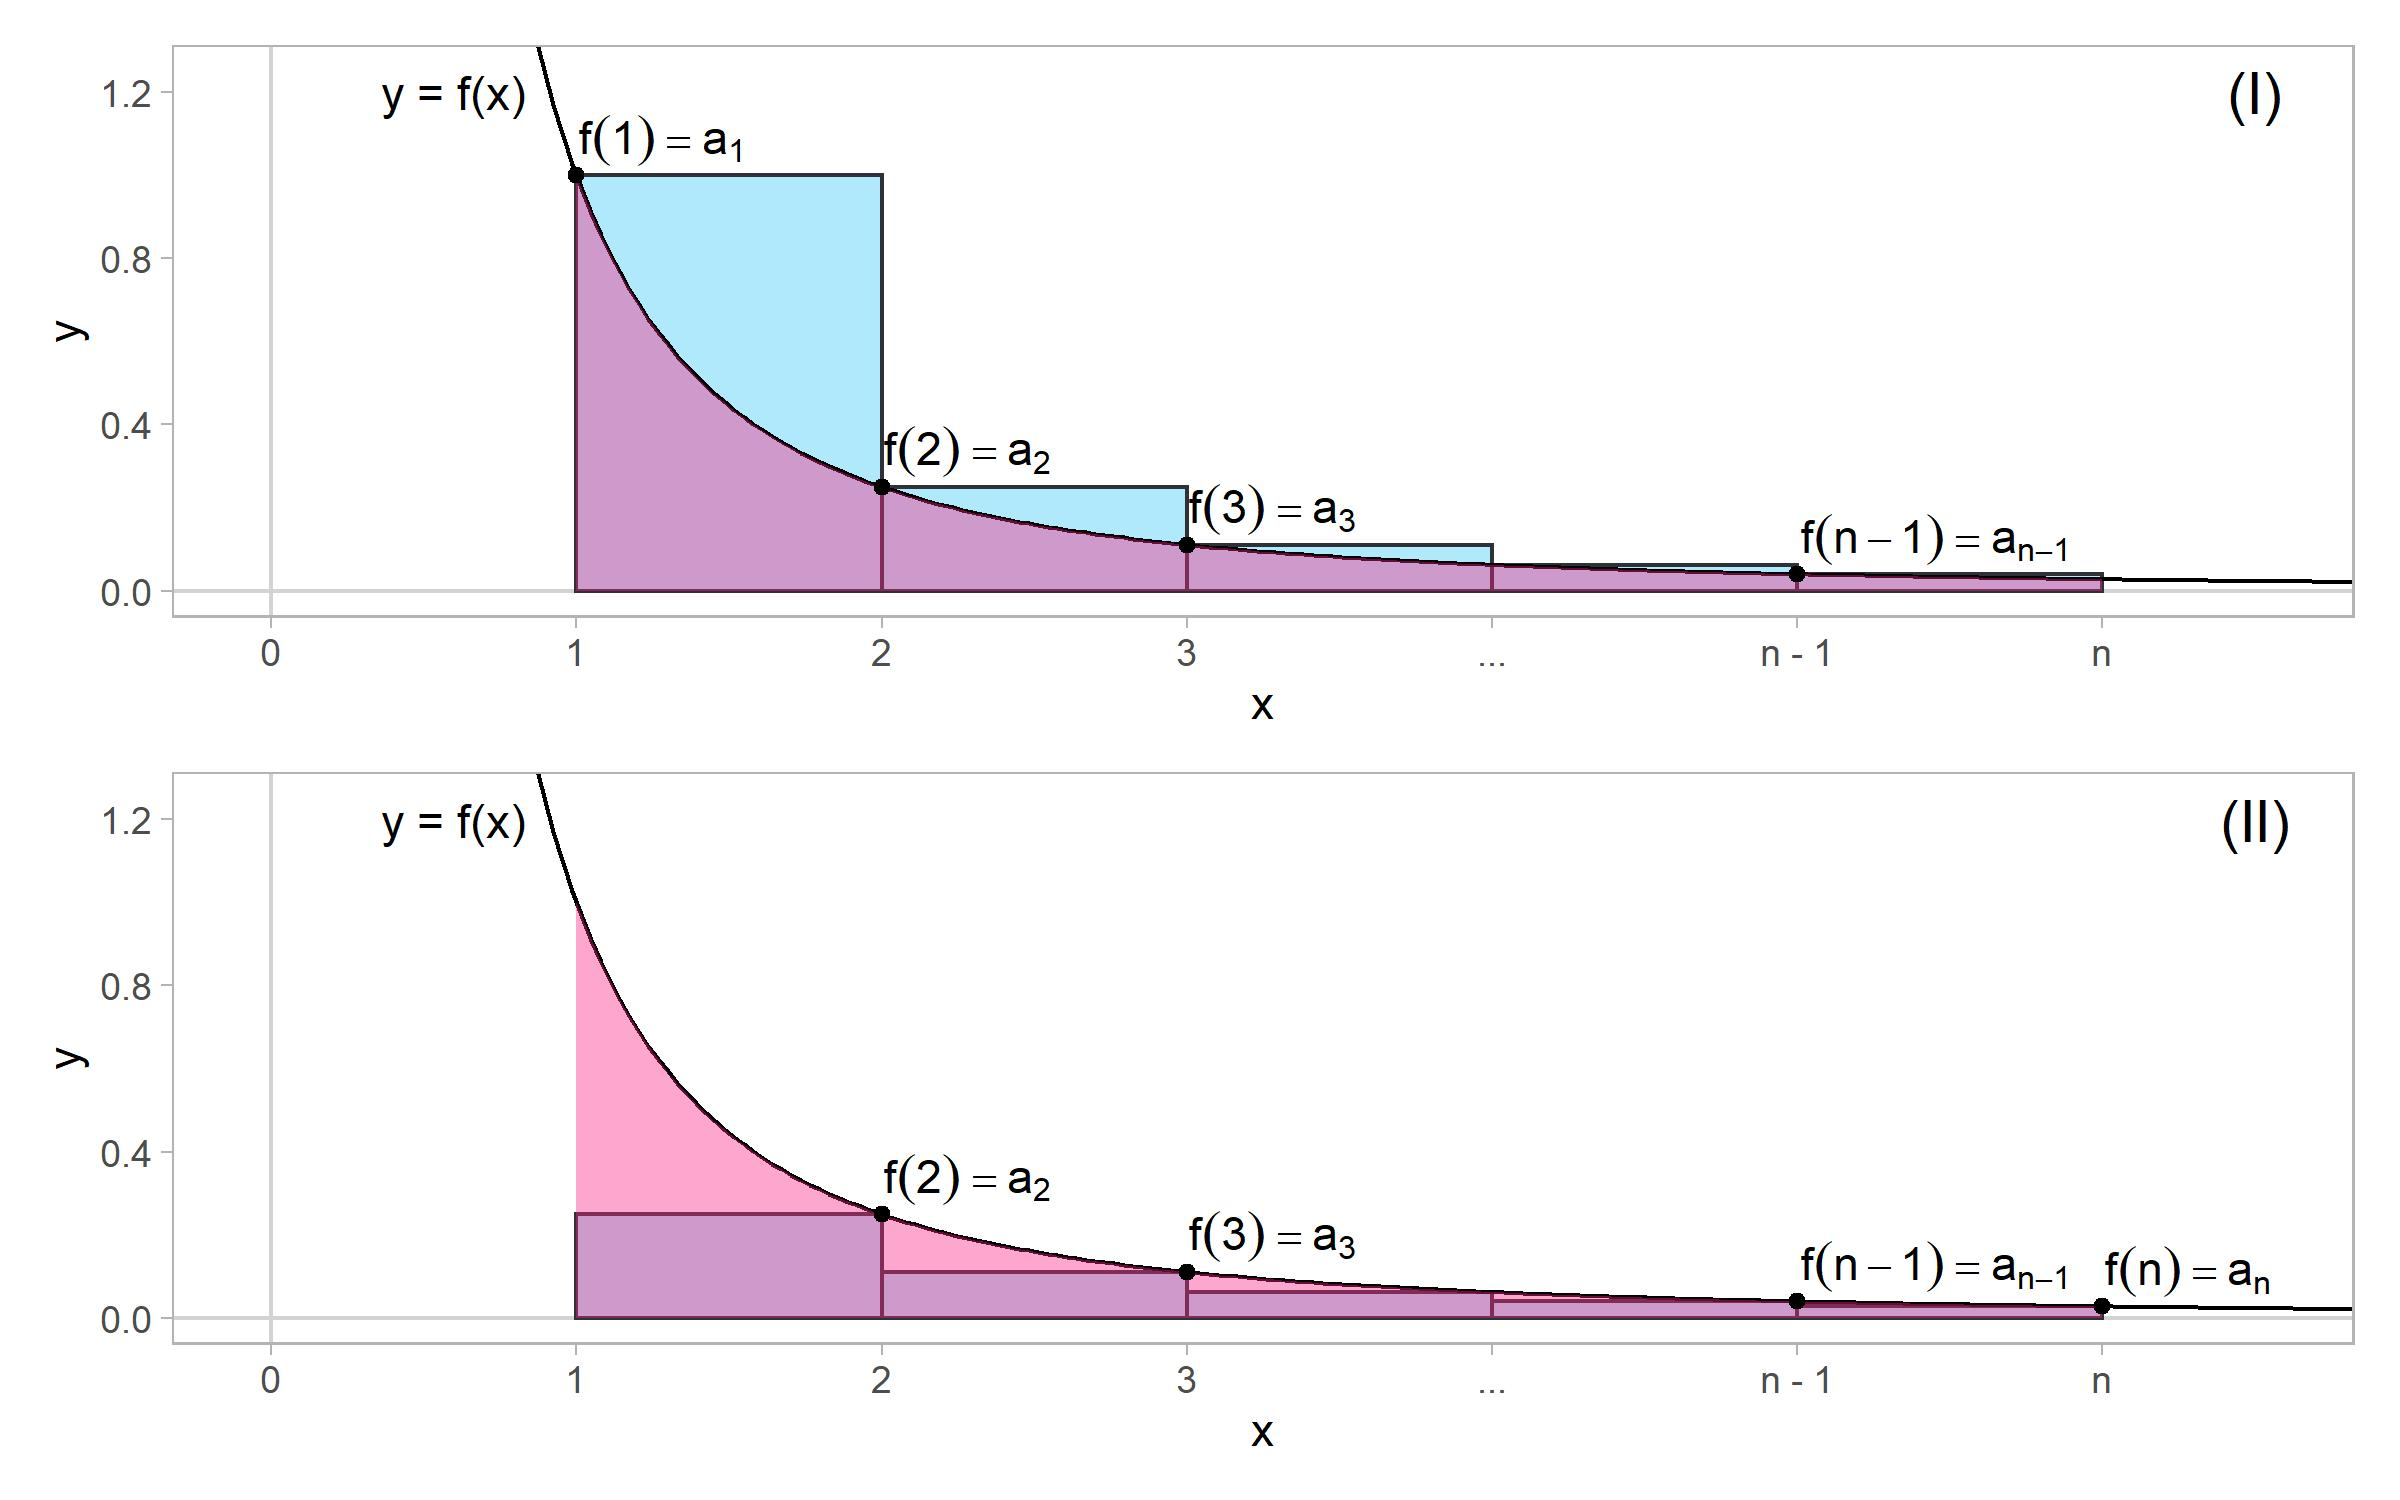
\includegraphics[scale=0.7]{int-test-plot.jpg}
\end{figure}

Mediante los gráficos (I) y (II) se puede estimar que el área bajo $f(x)$ entre $[1, \ n]$ es:
\[
  \sum_{i = 2}^{n} f(i) \Delta x \leq \int_{1}^{n} f(x)dx \leq \sum_{i = 1}^{n - 1} f(i) \Delta x
\]
donde $f(i) \cdot \Delta x$ es el área de los $(n - 1)$ rectángulos.

Debido a que $\Delta x = 1$ y $a_{n} = f(n)$, entonces
\[
  \sum_{i = 2}^{n} a_{i} \leq \int_{1}^{n} f(x)dx \leq \sum_{i = 1}^{n - 1} a_{i}
\]
Centrémonos en $\sum_{i = 2}^{n} a_{i} \leq \int_{1}^{n} f(x)dx$. Al sumar $a_{1} = f(1)$ en ella obtenemos que
\[
  a_{1} + \sum_{i = 2}^{n} a_{i} \leq a_{1} + \int_{1}^{n} f(x)dx
\]
Veamos que $a_{1} + \sum_{i = 2}^{n} a_{i} = \sum_{i = 1}^{n} a_{i} = s_{n}$, donde $s_{n}$ es la $n$-ésima \textbf{suma parcial} de $\sum_{n = 1}^{\infty} a_{n}$ cuyos términos están dados por $a_{n} = f(n)$, con $f(x)$ siendo no negativa y no creciente. Por lo tanto, $\{s_{n}\}$ es \textbf{monótona no decreciente} y tiene una cota inferior $m$ definida.
\[
  m \leq s_{n} \leq a_{1} + \int_{1}^{n} f(x)dx
\]
Por otra parte, como $f(x) \geq 0$, entonces $\int_{1}^{n} f(x)dx \leq \int_{1}^{\infty} f(x)dx$. Esto implica que:
\[
   m \leq s_{n} \leq a_{1} + \int_{1}^{\infty} f(x)dx
\]
Asumamos que $\int_{1}^{\infty} f(x)dx$ \textbf{converge} a un número $L$. Aquello significa que:
\[
  m \leq s_{n} \leq a_{1} + L
\]
Es decir, $\{s_{n}\}$ es \textbf{acotada} cuando $\int_{1}^{\infty} f(x)dx$ converge. Al ser \textbf{monótona} se puede concluir que es \textbf{convergente} y también lo es la serie dada por $a_{n} = f(n)$.

Ahora enfoquémonos en $\int_{1}^{n} f(x)dx \leq \sum_{i = 1}^{n - 1} a_{i}$, la que también se puede expresar como
\[
  \int_{1}^{n} f(x)dx \leq s_{n - 1}
\]
donde $s_{n - 1}$ es la $(n - 1)$ suma parcial de $\sum_{n = 1}^{\infty} a_{i}$ con términos $f(n) = a_{n} \geq 0$.

Supongamos que $\int_{1}^{\infty} f(x)dx$ \textbf{diverge}. Como $f(x) \geq 0$, lo anterior significa que
\[
  \int_{1}^{\infty} f(x)dx = \infty
\]
Por lo tanto, a medida que $n \to \infty$, $\{s_{n - 1}\}$ será \textbf{divergente} ya que $s_{n - 1} \geq \int_{1}^{n} f(x)dx$ y \textbf{la integral diverge} en este contexto. Además, como
\[
  s_{n - 1} \leq s_{n}
\]
debido a que $\sum_{n = 1}^{\infty} a_{n}$ es no negativa, $\{s_{n}\}$ será \textbf{divergente} y también esta serie.

Así, damos por demostrado que

\begin{enumerate}
\item Cuando $\int_{N}^{\infty}f(x)dx$ \textbf{converge}, $\sum_{n = N}^{\infty} a_{n}$ \textbf{converge}.
\item Cuando $\int_{N}^{\infty}f(x)dx$ \textbf{diverge}, $\sum_{n = N}^{\infty} a_{n}$ \textbf{diverge}.
\end{enumerate}

\subsubsection{Demostración de la prueba de convergencia de una serie \textit{p}.}

En la sección 2.3 se señaló que es posible demostrar la prueba de convergencia de una serie $p$ mediante la prueba de la integral. Veámoslo a continuación.

Como vimos anteriormente, una serie $p$ es de la forma
\[
  \sum_{n = 1}^{\infty} \frac{1}{n^{p}} = \frac{1}{1^{p}} + \frac{1}{2^{p}} + \frac{1}{3^{p}} + \cdots
\]
y se caracteriza por ser convergente cuando $p > 1$ y divergente cuando $p \leq 1$.

Establezcamos que $f(x) = 1/x^{p}$, lo que significa que $f(n) = 1/n^{p}$ para todo $n \in \mathbb{Z}$.

Es posible observar que, para todo $x \geq 1$, $f(x) \geq 0$, continua y no creciente. Esta última característica se puede verificar a partir de su derivada.
\[
  \frac{d}{dx} \left(\frac{1}{x^{p}}\right) = \frac{d}{dx} x^{-p}
                                            = -px^{-p - 1}
                                            = -px^{-(p + 1)} 
                                            = - \frac{p}{x^{p + 1}} < 0; \quad \forall x \geq 1
\]
Así, podemos usar la prueba de la integral para evaluar la convergencia de una serie $p$ mediante
\[
  \int_{1}^{\infty} \frac{1}{x^{p}} dx
\]
Esta integral impropia de tipo 1 la vimos en la Clase 35 (págs. 5-6), donde para $p = 1$:
\[
  \int_{1}^{\infty} \frac{1}{x} dx = \lim_{b \to \infty} \int_{1}^{b} \frac{1}{x} dx
                                       = \lim_{b \to \infty} (\ln(b) - \ln(1))
                                       = \infty
\]
Y para cualquier $p$ se obtiene que:
\[
  \int_{1}^{\infty} \frac{1}{x^{p}} dx = \lim_{b \to \infty} \int_{1}^{b} \frac{1}{x^{p}} dx
                                       = \frac{1}{-p + 1} \cdot \left[\left(\lim_{b \to \infty} b^{-p + 1}\right) - 1 \right]
\]
En consecuencia,
\[
  \int_{1}^{\infty} \frac{1}{x^{p}} dx =
  \left\{
    \begin{aligned}
    \frac{1}{p - 1}, \quad \text{ si } p > 1 \\
    \infty, \quad \text{ si } p < 1
    \end{aligned}
  \right.
\]
ya que cuando $p > 1$, $\lim_{b \to \infty} b^{-p + 1} = 0$, mientras que $\lim_{b \to \infty} b^{-p + 1} = \infty$ para todo $p < 1$. Esto nos lleva a concluir, primero, que:

\begin{enumerate}
\item $\int_{1}^{\infty} (1/x^{p})dx$ es \textbf{convergente} cuando $p > 1$.
\item $\int_{1}^{\infty} (1/x^{p})dx$ es \textbf{divergente} cuando $p \leq 1$.
\end{enumerate}

Y, en segundo lugar, que:

\begin{enumerate}
\item $\sum_{n = 1}^{\infty} 1/n^{p}$ es \textbf{convergente} cuando $p > 1$.
\item $\sum_{n = 1}^{\infty} 1/n^{p}$ es \textbf{divergente} cuando $p \leq 1$.
\end{enumerate}

como consecuencia de la \textbf{prueba de la integral}.

\subsection{Pruebas por comparación directa y del límite.}

Una debilidad de la prueba de la integral, es que no siempre es fácil o posible obtener su antiderivada. No obstante, otra opción para evaluar la convergencia de una serie es \textbf{comparándola} con otra semejante a ella y que sabemos que converge o diverge. Este método se conoce como \textbf{Prueba por comparación} y se divide en dos: Directa y Del límite.

\subsubsection{Comparación directa.}

Sean $\sum_{n = 1}^{\infty} a_{n}$ y $\sum_{n = 1}^{\infty} b_{n}$ dos series no negativas. Cuando
\[
  0 < a_{n} \leq b_{n}; \ \forall n \in \mathbb{Z}^{+}
\]
podemos aplicar la \textbf{Prueba por comparación directa}, la que señala que:

\begin{itemize}
\item Si $\sum_{n = 1}^{\infty} b_{n}$ \textbf{converge}, entonces $\sum_{n = 1}^{\infty} a_{n}$ también \textbf{converge}.
\item Si $\sum_{n = 1}^{\infty} a_{n}$ \textbf{diverge}, entonces $\sum_{n = 1}^{\infty} b_{n}$ también \textbf{diverge}.
\end{itemize}

Una forma más intuitiva de recordar la prueba por comparación directa, es la que sigue:

\begin{itemize}
\item Si la serie \textbf{más grande converge}, entonces la \textbf{más chica converge}.
\item Si la serie \textbf{más chica diverge}, entonces la \textbf{más grande converge}.
\end{itemize}

\textbf{Demostración.} Sean $\sum_{n = 1}^{\infty} a_{n}$ y $\sum_{n = 1}^{\infty} b_{n}$ dos series con $0 \leq a_{n} \leq b_{n}$ para todo $n \in \mathbb{Z}^{+}$, donde
\[
  s_{n} = \sum_{i = 1}^{n} a_{n} \quad \text{y} \quad t_{n} = \sum_{i = 1}^{n} b_{n}
\]
En ese sentido, tanto $\{s_{n}\}$ como $\{t_{n}\}$ son monótonas no decrecientes y $s_{n} \leq t_{n}$ para todo entero positivo $n$.

Para la primera parte de la prueba por comparación directa, asuma que $\sum_{n = 1}^{\infty} b_{n}$ \textbf{converge}. Es decir,
\[
  \sum_{n = 1}^{\infty} b_{n} = L
\]
donde $L$ es un valor finito.

Debido a que $\{s_{n}\}$ es monótona no decreciente, entonces tiene una cota inferior $m$. Sumado al hecho de que $s_{n} \leq t_{n}$, entonces:
\[
  m \leq s_{n} \leq t_{n} \leq L
\]
Como vemos, $L$ es una cota superior de $\{s_{n}\}$, lo que significa que es \textbf{convergente} y también lo es la $\sum_{n = 1}^{\infty} a_{n}$. Es decir,

\begin{center}
$\sum_{n = 1}^{\infty} a_{n}$ es \textbf{convergente} cuando también lo es $\sum_{n = 1}^{\infty} b_{n}$.
\end{center}

Ahora demostremos la segunda parte de la prueba por comparación directa asumiendo que $\sum_{n = 1}^{\infty} a_{n}$ \textbf{diverge}. Esto implica que $\{s_{n}\}$ también lo hace.

Puesto que $s_{n} \leq t_{n}$, si $\{s_{n}\}$ \textbf{diverge}, aquello también sucede con $\{t_{n}\}$. En consecuencia, $\sum_{n = 1}^{\infty} b_{n}$ es \textbf{divergente} y concluimos que:

\begin{center}
$\sum_{n = 1}^{\infty} b_{n}$ es \textbf{divergente} cuando también lo es $\sum_{n = 1}^{\infty} a_{n}$.
\end{center}

De este modo, damos por demostrado la prueba por comparación directa.

\subsubsection{Comparación del límite.}

Sean dos series no negativas $\sum_{n = 1}^{\infty} a_{n}$ y $\sum_{n = 1}^{\infty} b_{n}$. La \textbf{prueba por comparación del límite} señala

\begin{enumerate}
\item Si $\displaystyle \lim_{n \to \infty} \frac{a_{n}}{b_{n}} = L$, para $0 < L < \infty$, entonces $\sum_{n = 1}^{\infty} a_{n}$ y $\sum_{n = 1}^{\infty} b_{n}$ \textbf{convergen o divergen al mismo tiempo}.
\item Si $\displaystyle \lim_{n \to \infty} \frac{a_{n}}{b_{n}} = 0$ y $\sum_{n = 1}^{\infty} b_{n}$ \textbf{converge}, entonces $\sum_{n = 1}^{\infty} a_{n}$ \textbf{converge}.
\item Si $\displaystyle \lim_{n \to \infty} \frac{a_{n}}{b_{n}} = \infty$ y $\sum_{n = 1}^{\infty} b_{n}$ \textbf{diverge}, entonces $\sum_{n = 1}^{\infty} a_{n}$ \textbf{diverge}.
\end{enumerate}

\textbf{Demostración parte 1.}\footnote{No pude ubicar una demostración para las partes 2 y 3 de esta prueba. En el texto de Thomas la dejan como tarea, así que algún día intentaré hacerlo (o quizá la encuentre por ahí).} Sean dos sucesiones infinitas $\{a_{n}\}$ y $\{b_{n}\}$ tal que, para todo $n \in \mathbb{Z}^{+}$, $a_{n}, \ b_{n} \geq 0$ y se cumple que
\[
  \lim_{n \to \infty} \frac{a_{n}}{b_{n}} = L, \text{ con } 0 < L < \infty
\]
Debido a que existe el límite de $(a_{n}/b_{n})$, eso quiere decir que para un número $\epsilon > 0$ existe un correspondiente entero $N$ tal que, para todo $n > N$,\footnote{Esto corresponde a la definición precisa del límite de una sucesión.}
\[
  \left|\frac{a_{n}}{b_{n}} - L \right| < \epsilon
\]
Por las propiedades de las desigualdades de los valores absolutos, la que se encuentra arriba podemos expresarla como:
\[
  -\epsilon < \frac{a_{n}}{b_{n}} - L < \epsilon
\]
Al sumar $L$ y al multiplicar por $b_{n}$ a esta desigualdad compuesta, obtenemos lo siguiente:
\[
  (L - \epsilon) b_{n} < a_{n} < (L + \epsilon) b_{n}
\]
En $a_{n} < (L + \epsilon) b_{n}$, si $\sum_{n = 1}^{\infty} b_{n}$ \textbf{converge}, entonces también lo hace $\sum_{n = 1}^{\infty} (L + \epsilon) b_{n}$. Esto implica por la \textbf{prueba por comparación directa} que $\sum_{n = 1}^{\infty} a_{n}$ es \textbf{convergente}.

Por otra parte, en $(L - \epsilon) b_{n} < a_{n}$, si $\sum_{n = 1}^{\infty} a_{n}$ \textbf{diverge}, por la \textbf{prueba por comparación directa} $\sum_{n = 1}^{\infty} b_{n}$ también es \textbf{divergente}.

A partir de los dos últimos párrafos podemos concluir que si
\[
  \lim_{n \to \infty} \frac{a_{n}}{b_{n}} = L; \text{ donde } 0 < L < \infty
\]
las series no negativas $\sum_{n = 1}^{\infty} a_{n}$ y $\sum_{n = 1}^{\infty} b_{n}$ convergen o divergen al mismo tiempo (Q. E. D).

La ventaja de esta prueba con respecto a la de por comparación directa, es que no debemos revisar que cada término de una sucesión sean menores a todos los de la otra para aplicarla, lo que la hace más rápido de trabajar.


\section{Series alternantes.}

Es lógico pensar que no todas las series son no negativas. Una de ellas son las \textbf{Series alternantes} donde cada término es de signo distinto al anterior\footnote{Dicho de otro modo, los términos alternadamente son de signo opuesto.}. Algunos ejemplos son:
\[
  \sum_{n = 1}^{\infty} (-1)^{n - 1} a_{n} \quad \text{ o } \quad
  \sum_{n = 1}^{\infty} (-1)^{n} a_{n} \quad \text{ o } \quad
  \sum_{n = 1}^{\infty} (-1)^{n + 1} a_{n}
\]
Una serie alternante como las vistas arriba \textbf{converge} si cumple las siguientes condiciones\footnote{Estas condiciones se refieren a los términos de $\{a_{n}\}$ sin considerar el factor $(-1)^{n}$.}:

\begin{enumerate}
\item $0 < a_{n + 1} \leq a_{n}$, para todo $n$ (i.e, $\{a_{n}\}$ eventualmente debe ser \textbf{no creciente}).
\item $\displaystyle \lim_{n \to \infty} a_{n} = 0$.
\end{enumerate}

\subsection{Demostración de la convergencia de una serie alternante.}

Considere la siguiente serie alternante, con $0 < a_{n + 1} \leq a_{n}$ para todo $n \in \mathbb{Z}^{+}$.
\[
  \sum_{n = 1}^{\infty} (-1)^{n + 1} a_{n} = (a_{1} - a_{2}) + (a_{3} - a_{4}) + (a_{5} - a_{6}) + \ldots
\]
donde
\[
  \lim_{n \to \infty} a_{n} = 0
\]
Si bien no hay certeza sobre el signo del último término de esta serie, se puede observar que los de índice $2n$ siempre son negativos. Por este motivo, veamos sus \textbf{\textit{n} sumas parciales pares}, $s_{2n}$.

\begin{align*}
  s_{2} &= (a_{1} - a_{2}) \\
  s_{4} &= s_{2} + (a_{3} - a_{4}) \\
  s_{6} &= s_{4} + (a_{5} - a_{6}) \\
  \vdots \\
  s_{2n} &= s_{2n - 2} + (a_{2n - 1} - a_{2n})
\end{align*}
Debido a que $0 < a_{n + 1} \leq a_{n}$ veamos, por ejemplo, que:
\[
  (a_{2n - 1} - a_{2n}) > 0; \ \text{para todo } n
\]
Producto de aquello, $s_{2n - 2} \leq s_{2n}$ porque la suma entre cualquier valor positivo y $s_{2n - 2}$ será mayor a este último. Por lo tanto,
\[
  0 \leq s_{2} \leq s_{4} \leq s_{6} \leq \ldots \leq s_{2n}
\]
Es decir, $\{s_{2n}\}$ es una sucesión \textbf{monótona no decreciente} y, por consiguiente, tiene una cota inferior $m$.

La $n$-ésima suma parcial par
\[
  s_{2n} = (a_{1} - a_{2}) + (a_{3} - a_{4}) + \ldots + (a_{2n - 1} - a_{2n})
\]
también se puede escribir de la siguiente manera:
\[
  s_{2n} = a_{1} - (a_{2} - a_{3}) - (a_{4} - a_{5}) - \ldots - (a_{2n - 2} - a_{2n - 1}) - a_{2n}
\]
Las restas de los paréntesis son positivas y como cada $a_{n + 1} \leq a_{n}$, entonces:
\[
  m \leq s_{2n} \leq a_{1}
\]
En otras palabras, $a_{1}$ es la cota superior de $\{s_{2n}\}$. Así, por el Teorema de la sucesión monótona se puede afirmar que es \textbf{convergente}.
\[
  \lim_{n \to \infty} s_{2n} = L; \text{ con } L \leq a_{1} < \infty
\]
Ahora observemos las $n$ \textbf{sumas parciales impares}, $s_{2n + 1}$, la cual podemos escribir como
\[
  s_{2n + 1} = s_{2n} + a_{2n + 1}
\]
Para saber si la serie alternante es convergente a partir de las condiciones dadas inicialmente, necesitamos saber si las sumas parciales impares convergen al mismo valor de las pares. Por esta razón, tomemos el límite de $s_{2n + 1}$.
\[
  \lim_{n \to \infty} s_{2n + 1} = \lim_{n \to \infty} s_{2n} + \lim_{n \to \infty} a_{2n + 1}
\]
Sabemos que $\lim_{n \to \infty} s_{2n} = L$ y como $\lim_{n \to \infty} a_{n} = 0$, entonces $\lim_{n \to \infty} a_{2n + 1} = 0$. Así,
\[
  \lim_{n \to \infty} s_{2n + 1} = L + 0 = L
\]
Esta igualdad nos permite concluir que una serie alternante es \textbf{convergente} si:

\begin{enumerate}
\item $0 < a_{n + 1} \leq a_{n}$.
\item $\displaystyle \lim_{n \to \infty} a_{n} = 0$.
\end{enumerate}


\section{Convergencia absoluta de una serie.}

Hay ocasiones donde una serie puede tener términos negativos de manera irregular y ser divergente, pero al tomar el \textbf{valor absoluto} de éstos, la suma sí se aproxima a un valor finito. En esos casos decimos que es \textbf{absolutamente convergente}.

En general, se dice que $\sum_{n = 1}^{\infty} a_{n}$ es \textbf{absolutamente convergente} si $\sum_{n = 1}^{\infty} |a_{n}|$ es \textbf{convergente}, donde
\[
  \sum_{n = 1}^{\infty} |a_{n}| = |a_{1}| + |a_{2}| + |a_{3}| + |a_{4}| + \ldots
\]
Por otra parte, si $\sum_{n = 1}^{\infty} a_{n}$ es \textbf{convergente sin ser absolutamente convergente}, se señala que es \textbf{condicionalmente convergente}.

\subsection{Prueba de la convergencia absoluta.}

La \textbf{prueba de la convergencia absoluta} señala que si $\sum_{n = 1}^{\infty} |a_{n}|$ es convergente, entonces también lo es $\sum_{n = 1}^{\infty} a_{n}$. No obstante, el reverso de este criterio\footnote{Es decir, que una serie sea convergente debido a su convergencia absoluta.} no siempre es verdadero.

\textbf{Demostración.} Considere la serie
\[
  \sum_{n = 1}^{\infty} |a_{n}|
\]
En ese sentido, para todo $n \in \mathbb{Z}^{+}$
\[
  -|a_{n}| \leq a_{n} \leq |a_{n}|
\]
Al sumar $|a_{n}|$ en esta desigualdad obtenemos que
\[
  0 \leq a_{n} + |a_{n}| \leq 2|a_{n}|
\]
Si $\sum_{n = 1}^{\infty} |a_{n}|$ converge, entonces también lo hace $\sum_{n = 1}^{\infty} 2|a_{n}|$. En consecuencia, por la prueba por comparación directa\footnote{Podemos aplicar este criterio porque tanto $\sum_{n = 1}^{\infty} 2|a_{n}|$ como $\sum_{n = 1}^{\infty} (a_{n} + |a_{n}|)$ son no negativas.}, $\sum_{n = 1}^{\infty} (a_{n} + |a_{n}|)$ será \textbf{convergente}.

Observemos que la serie
\[
  \sum_{n = 1}^{\infty} a_{n} = \sum_{n = 1}^{\infty} (a_{n} + |a_{n}|) - \sum_{n = 1}^{\infty} |a_{n}|
\]
Así, se concluye que $\sum_{n = 1}^{\infty} a_{n}$ es \textbf{convergente} porque es la diferencia de dos series que también lo son (Q. E. D).

\subsection{Prueba de la razón.}

Podría ser de nuestro interés conocer la tasa de crecimiento o caída de una serie. Para ello, podemos usar la \textbf{prueba de la razón}.

Sea $\sum_{n = 1}^{\infty} a_{n}$ una serie con $a_{n} \neq 0$ para todo $n$, donde
\[
  \lim_{n \to \infty} \left|\frac{a_{n + 1}}{a_{n}}\right| = L
\]
La \textbf{prueba de la razón} indica que

\begin{enumerate}
\item Si $L < 1$, entonces $\sum_{n = 1}^{\infty} a_{n}$ es \textbf{absolutamente convergente}.
\item Si $L > 1$ o $L = \infty$, entonces $\sum_{n = 1}^{\infty} a_{n}$ es \textbf{divergente}.
\item Si $L = 1$, \textbf{la prueba no es concluyente} porque no permite afirmar si la serie es convergente o divergente.
\end{enumerate}

\textbf{Demostración parte 1.} Sea $\sum_{n = 1}^{\infty} a_{n}$ una serie con $a_{n} \neq 0$ para todo $n$ donde
\[
  \lim_{n \to \infty} \left|\frac{a_{n + 1}}{a_{n}}\right| = L < 1
\]
Lo señalado arriba implica que para un $\epsilon > 0$ existe un $N$ tal que, para todo $n \geq N$,
\begin{gather*}
  \left|\frac{a_{n + 1}}{a_{n}} - L \right| < \epsilon \\
  - \epsilon < \left|\frac{a_{n + 1}}{a_{n}} - L \right| < \epsilon \\
  L - \epsilon < \left|\frac{a_{n + 1}}{a_{n}}\right| < L + \epsilon
\end{gather*}
De aquí en adelante asumamos que escogimos un $\epsilon$ tal que $L + \epsilon < 1$.

Ahora centrémonos en $|(a_{n + 1}/a_{n})| < L + \epsilon$ y multipliquémosla por $|a_{n}|$.
\[
  |a_{n + 1}| < |a_{n}| (L + \epsilon) 
\]
Digamos que $n = N$. En la desigualdad de arriba implica que
\[
  |a_{N + 1}| < |a_{N}| (L + \epsilon)
\]
Luego, cuando $n = N + 1$, obtenemos que
\begin{align*}
  |a_{(N + 1) + 1}| &< |a_{N + 1}| (L + \epsilon) \\
        |a_{N + 2}| &< |a_{N + 1}| (L + \epsilon) < [(L + \epsilon) |a_{N}|] (L + \epsilon) \\
        |a_{N + 2}| &< |a_{N + 1}| (L + \epsilon) < |a_{N}| (L + \epsilon)^{2}
\end{align*}
En otras palabras:

\begin{table}[!hbt]
\centering

\begin{tabular}{c | c}
$n$ & $|a_{n + 1}| < |a_{n}| (L + \epsilon)$ \\
\hline
    $N$ & $|a_{N + 1}| < |a_{N}| (L + \epsilon)$  \\
$N + 1$ & $|a_{N + 2}| < |a_{N}| (L + \epsilon)^{2}$ \\
$N + 2$ & $|a_{N + 3}| < |a_{N}| (L + \epsilon)^{3}$ \\
$\vdots$ & $\vdots$ \\
$N + C$ & $|a_{N + (C + 1)}| < |a_{N}| (L + \epsilon)^{(C + 1)}$
\end{tabular}

\end{table}

con $C =$ constante.

Establezcamos que $C + 1 = K$, otra constante. Por lo tanto,
\[
  |a_{N + K}| < |a_{N}| (L + \epsilon)^{K}
\]
Ahora, consideremos las series
\[
  \text{(I)} \ \sum_{K = 1}^{\infty} |a_{N + K}|
  \qquad \text{y} \qquad
  \text{(II)} \ \sum_{K = 1}^{\infty} |a_{N}| (L + \epsilon)^{K}
\]
Observemos que (II) es una \textbf{serie geométrica}. Debido a que su razón común $(L + \epsilon) < 1$, entonces es \textbf{convergente}.

Por otra parte, como $0 < |a_{N + K}| < |a_{N}| (L + \epsilon)^{K}$ para todo $K$, por la \textbf{prueba por comparación directa} la serie (I) es \textbf{convergente}.

En general, la propiedad de convergencia o divergencia de una serie \textbf{no se altera al añadir o quitar términos} de ella. En ese sentido, es válido señalar que:
\[
  \sum_{K = 1}^{\infty} |a_{N + K}| = \sum_{n = 1}^{\infty} |a_{n}|
\]
La igualdad de arriba implica que $\sum_{n = 1}^{\infty} |a_{n}|$ es \textbf{convergente}. Así, por la \textbf{prueba de la convergencia absoluta}, $\sum_{n = 1}^{\infty} a_{n}$ es \textbf{absolutamente convergente} (Q. E. D).

\textbf{Demostración parte 2.} Considere la serie $\sum_{n = 1}^{\infty} a_{n}$ con $a_{n} \neq 0$ para todo $n$ donde
\[
  \lim_{n \to \infty} \left|\frac{a_{n + 1}}{a_{n}}\right| = L; \ \text{tal que } 1 < L \leq \infty
\]
Si $L$ toma un valor en $(1, \ \infty]$, significa que eventualmente para todo $n \geq N$,
\begin{align*}
  \left|\frac{a_{n + 1}}{a_{n}}\right| &> 1 \\
                           |a_{n + 1}| &> |a_{n}|
\end{align*}
Es decir, cada término de $\{a_{n}\}$ será mayor a su antecesor. En consecuencia,
\[
  \lim_{n \to \infty} a_{n} \neq 0
\]
Por la \textbf{prueba del \textit{n}-ésimo término}, la serie $\sum_{n = 1}^{\infty} a_{n}$ es \textbf{divergente} (Q. E. D).

\textbf{Demostración parte 3.} Para ver que la prueba de la razón falla cuando $L = 1$, considere las siguientes series $p$.
\[
  \text{(I) } \sum_{n = 1}^{\infty} \frac{1}{n}
  \qquad \qquad
  \text{(II) } \sum_{n = 1}^{\infty} \frac{1}{n^{2}}
\]
Calculemos el límite de la razón $|(a_{n + 1}/a_{n})|$ en las sucesiones de las dos series vistas arriba.
\begin{align*}
  &\text{(I) } \lim_{n \to \infty} \frac{1/(n + 1)}{1/n} = \lim_{n \to \infty} \frac{1}{n + 1} \cdot \frac{n}{1}
                                                         = \lim_{n \to \infty} \frac{n}{n + 1}
                                                         = \lim_{n \to \infty} \frac{1}{1 + (1/n)}
                                                         = 1 \\
  &\text{(II) } \lim_{n \to \infty} \frac{1/(n^{2} + 1)}{1/n^{2}} = \lim_{n \to \infty} \frac{1}{n^{2} + 1} \cdot \frac{n^{2}}{1}
                                                                  = \lim_{n \to \infty} \frac{n^{2}}{n^{2} + 1}
                                                                  = \lim_{n \to \infty} \frac{1}{1 + (1/n^{2})}
                                                                  = 1
\end{align*}
Los límites de la razón para los términos de ambas series son iguales a $1$. Sin embargo, estudiamos anteriormente que la serie (I) es divergente (serie armónica), mientras que (II) es convergente porque $p = 2 > 1$. Esto muestra la falla de la prueba de la razón cuando $L = 1$.

\subsection{Prueba de la raíz.}

Cuando los términos de una serie involucran \textbf{potencias}, el criterio más apropiado para evaluar si converge o diverge es la \textbf{prueba de la raíz}.

Sea $\sum_{n = 1}^{\infty} a_{n}$ una serie donde ocurre que
\[
  \lim_{n \to \infty} \sqrt[n]{|a_{n}|} = L
\]
La prueba de la raíz señala que:

\begin{enumerate}
\item Si $L < 1$, entonces $\sum_{n = 1}^{\infty} a_{n}$ es \textbf{absolutamente convergente}.
\item Si $1 < L \leq \infty$, entonces $\sum_{n = 1}^{\infty} a_{n}$ es \textbf{divergente}.
\item Si $L = 1$, se concluye que \textbf{la prueba no es concluyente}.
\end{enumerate}

Como veremos a continuación, la demostración de la prueba de la raíz es similar a la de la razón estudiada en la sección anterior.

\textbf{Demostración parte 1.} Sea $\sum_{n = 1}^{\infty} a_{n}$ una serie donde el límite de sus términos es
\[
  \lim_{n \to \infty} \sqrt[n]{|a_{n}|} = L < 1
\]
Debido a que existe el límite de arriba, para un $\epsilon > 0$ existe un entero $N > 0$ tal que, para todo $n \geq N$,

\begin{gather*}
  |\sqrt[n]{|a_{n}|} - L| < \epsilon \\
  L - \epsilon < \sqrt[n]{|a_{n}|} < L + \epsilon
\end{gather*}
Asumamos que $L + \epsilon < 1$. Si a $\sqrt[n]{|a_{n}|} < L + \epsilon < 1$ la elevamos a $n$, obtenemos que:
\[
  |a_{n}| < (L + \epsilon)^{n} < 1; \ \forall n \geq N
\]
De este modo, consideremos las series
\[
  \text{(I) } \sum_{n = N}^{\infty} (L + \epsilon)^{n} \qquad \qquad
  \text{(II) } \sum_{n = N}^{\infty} |a_{n}|
\]
La serie (I) es una geométrica y \textbf{convergente}, ya que su razón común es $(L + \epsilon)^{n} < 1$. En ese sentido, a partir de la \textbf{prueba por comparación directa}, la serie (II) también es \textbf{convergente}.

La serie (II) podemos escribirla como parte de otra suma de los mismos términos:
\[
  \sum_{n = 1}^{\infty} |a_{n}| = \sum_{n = 1}^{N - 1} |a_{n}| + \sum_{n = N}^{\infty} |a_{n}|
\]
Como añadir términos a una serie no altera su propiedad de convergencia, entonces $\sum_{n = 1}^{\infty} |a_{n}|$ es convergente y, por la \textbf{prueba de la convergencia absoluta}, $\sum_{n = 1}^{\infty} a_{n}$ es \textbf{absolutamente convergente} (Q. E. D).

\textbf{Demostración parte 2.} Sea $\sum_{n = 1}^{\infty} a_{n}$ una serie donde
\[
  \lim_{n \to \infty} \sqrt[n]{|a_{n}|} = L > 1
\]
El límite de arriba implica que, eventualmente para todo $n \geq N \in \mathbb{Z}^{+}$,
\begin{align*}
  \sqrt[n]{|a_{n}|} > 1 \\
  |a_{n}| > 1
\end{align*}
Es decir, todos los términos de $\{|a_{n}|\}$ serán mayores a $1$. Esto implica que:
\[
  \lim_{n \to \infty} |a_{n}| \neq 0
\]
Así, por la \textbf{prueba del \textit{n}-ésimo término}, la serie $\sum_{n = 1}^{\infty} a_{n}$ es \textbf{divergente} (Q. E. D).

\textbf{Demostración parte 3.} Considere las series $p$
\[
  \text{(I) } \sum_{n = 1}^{\infty} \frac{1}{n} \qquad \qquad \text{(II) } \sum_{n = 1}^{\infty} \frac{1}{n^{2}}
\]
Calculemos el límite de la raíz $n$-ésima de los términos de (I) y (II).
\begin{align*}
&\text{(I) } \lim_{n \to \infty} \sqrt[n]{\frac{1}{n}} = \lim_{n \to \infty} \frac{\sqrt[n]{1}}{\sqrt[n]{n}}
                                                       = \frac{1}{1}
                                                       = 1 \\
&\text{(II) } \lim_{n \to \infty} \sqrt[n]{\frac{1}{n^{2}}} = \lim_{n \to \infty} \frac{\sqrt[n]{1}}{\sqrt[n]{n^{2}}}
                                                       = \frac{1}{1}
                                                       = 1
\end{align*}
Como vemos, tanto en (I) como en (II) el límite de las raíces $n$-ésima de sus términos es igual a $1$. Sin embargo, sabemos que (I) es divergente y (II) es convergente, de manera que \textbf{la prueba falla en evaluar estos criterios}.
\end{document}
